\begin{figure*}[!htbp]
\centering
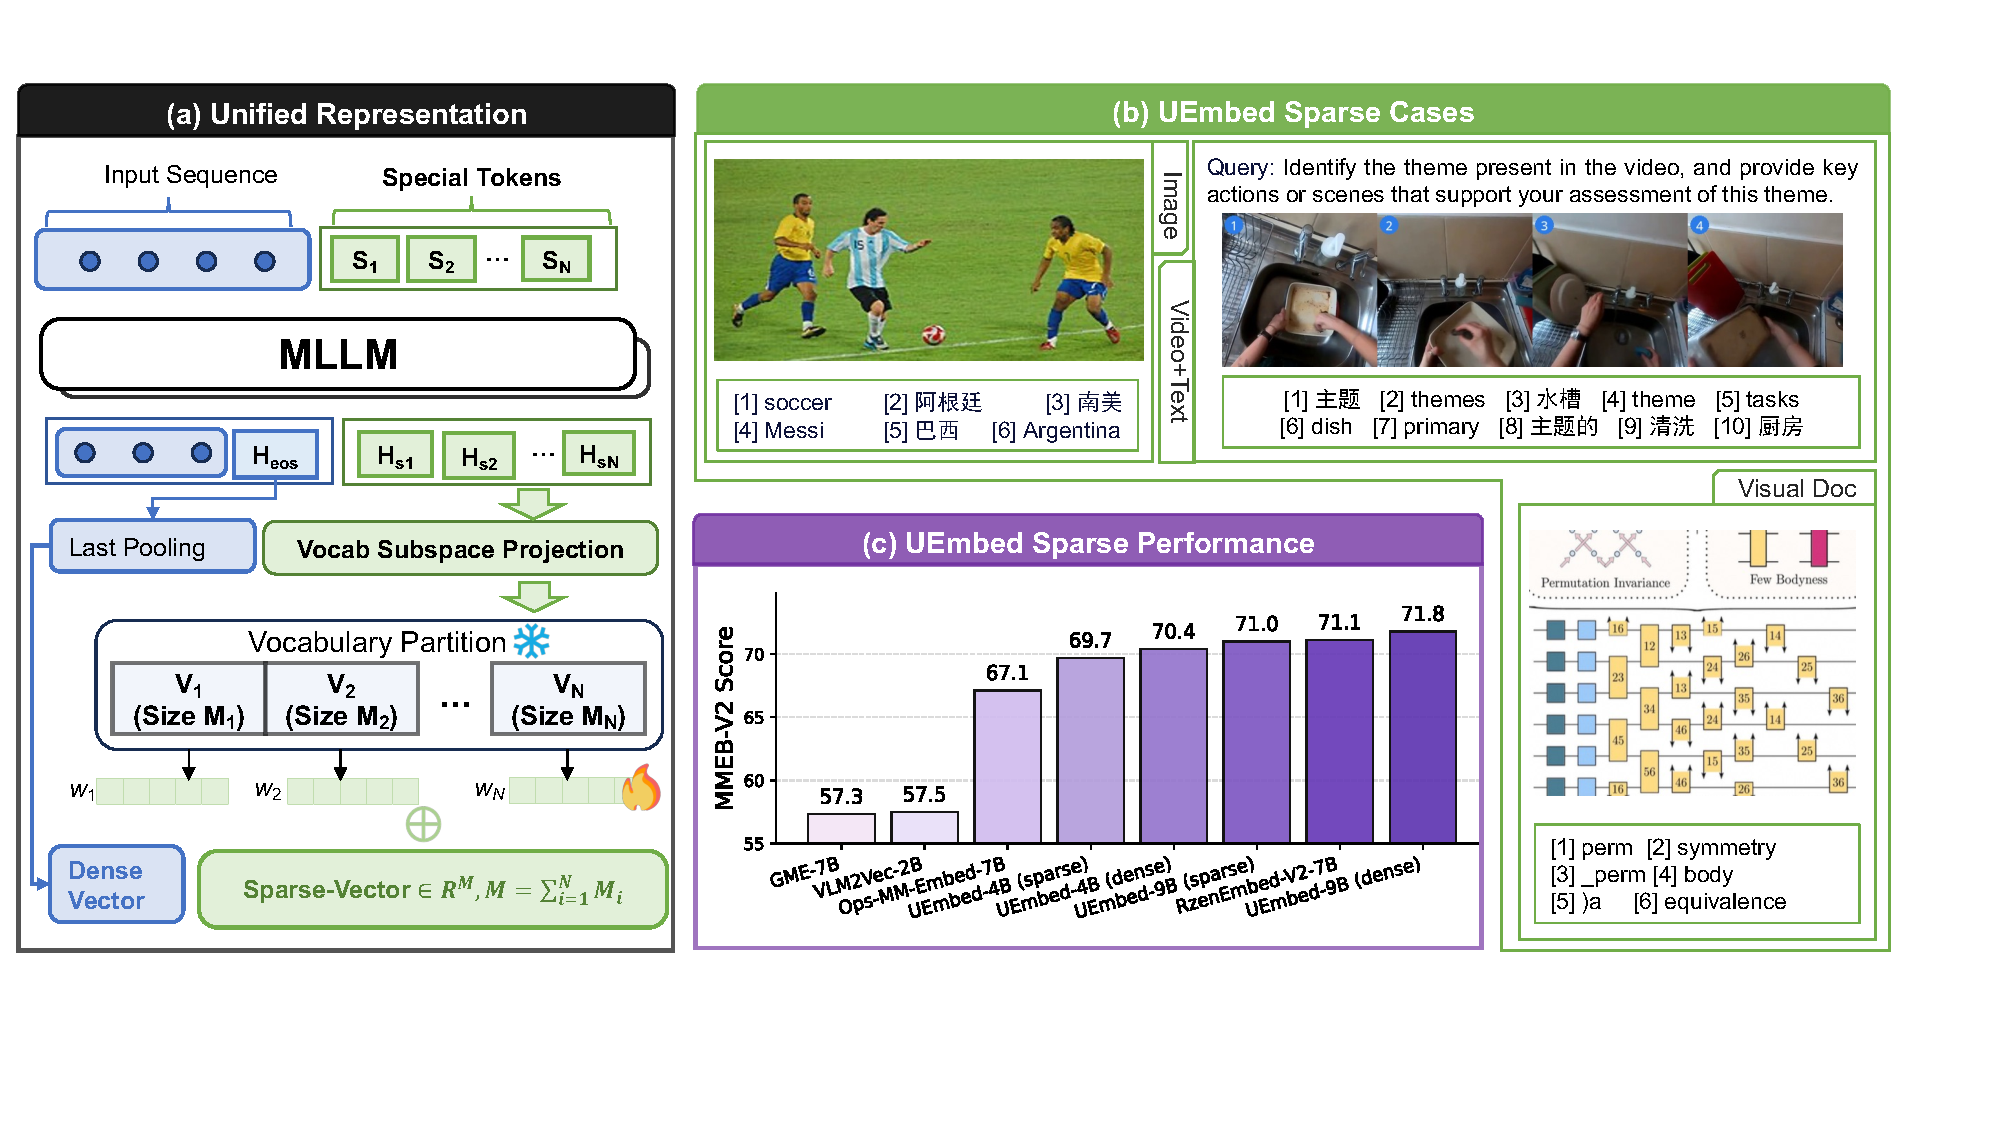
\includegraphics[width=0.90\linewidth]{resources/arxiv-figure1.pdf}
\caption{Overview of \ours. (a) Framework: we append $N$ learnable special tokens to a decoder-only MLLM and assign each token a disjoint vocabulary subset. (b) Sparse cases: examples of activated lexical tokens produced by \ours-9B. (c) Performance: \ours achieves strong sparse and dense retrieval results on MMEB-v2.}
\label{fig:arxiv-figure1}
\end{figure*}


\section{Introduction}
\label{sec:intro}

Information retrieval (IR) underpins a broad range of real-world applications, including web search and question answering. 
Sparse lexical methods such as BM25~\citep{bm25} remain widely deployed for their efficiency and interpretability, but their reliance on exact term matching limits their ability to capture semantic similarity beyond surface-level lexical overlap.
Learned sparse retrieval (LSR) addresses this gap by training neural models to produce sparse lexical representations.
Representative methods such as SPLADE~\citep{spladev1, spladev2, spladepp} combine token-level transformations with max pooling, substantially improving retrieval quality over classical term-weighting schemes.

Despite this progress, LSR remains limited in three key respects.
(1) \emph{Architectural constraint:} current LSR methods are largely built on encoder-style, bidirectional architectures (\eg BERT~\citep{bert}). Due to the causal masking of unidirectional attention, decoder-only models cannot directly reuse traditional pooling strategies to capture the global context needed for sparse representations. 
Leveraging large language models (LLMs) for sparse retrieval has typically required either converting the causal backbone to a bidirectional one~\citep{bgem3} or adopting dedicated training curricula~\citep{laconic}, both of which incur additional training cost and break compatibility with optimized causal-model serving frameworks such as vLLM~\citep{vllm}.  
(2) \emph{Limited modality:} most LSR methods remain confined to text, as traditional approaches rely heavily on text-only BERT architectures that lack native multimodal capabilities. 
The few multimodal methods~\citep{visualsparta, stair} introduce auxiliary cross-modal modules rather than deriving sparse representations directly from a single multimodal backbone, making them difficult to extend to new modalities.
(3) \emph{Unexplored practical utility:} existing sparse methods are predominantly evaluated on traditional benchmarks such as COCO~\citep{coco}, leaving the practical advantages of sparse retrieval under-examined beyond accuracy. 

The primary challenge in deriving sparse representations from causal models is the information bottleneck: relying on a single token (\eg EOS, CLS) to project into a massive $|V|$-dimensional vocabulary space severely limits representational capacity. To overcome this, we present \ours (\textbf{\underline{U}}nified \textbf{\underline{Embed}}ding), which appends $N$ learnable special tokens to an MLLM and assigns each token a disjoint subset of the vocabulary. Specifically, these subsets are derived via $k$-means clustering, which explicitly encourages each token to represent a distinct spatial direction. Under causal attention, each special token summarizes the input from its position and predicts sparse weights over its assigned cluster. The $N$ subsets are then concatenated into the full sparse vector. This partitioned projection effectively circumvents the single-token representational bottleneck. The dense embedding is obtained from the hidden state of the EOS token preceding the special tokens.    
As shown in~\autoref{fig:arxiv-figure1}(b), \ours produces semantically meaningful lexical activations, indicating that the sparse representation captures cross-modal semantics.

We evaluate \ours on text and multimodal embedding benchmarks, with results summarized in~\autoref{fig:arxiv-figure1}(c).
On MMEB-v2, \ours-9B reaches 71.8 (dense) and 71.0 (sparse), closing the gap between the two modes to within one point at every scale we test.
On BEIR (9 datasets, nDCG@10), \ours remains competitive with strong dense and sparse baselines such as SPLADE-v3~\citep{spladev3}.
Moreover, our analysis surfaces three practical advantages of \ours. First, hybrid scoring over its dense and sparse modes consistently improves text and visual-document retrieval. Second, its design retains compatibility with high-throughput serving stacks (\eg vLLM) and inverted-index search. Finally, on BrowseComp-Plus~\citep{browsecompplus}, the sparse mode reduces tool-call costs while maintaining comparable recall. 

We summarize our contributions as follows:
\begin{itemize} [leftmargin=*]
\itemsep0em
    \item We propose \ours, which produces both sparse and dense retrieval representations from a single decoder-only backbone. 
    \item \ours unifies different modalities in one model and can be easily extended to diverse modality settings. To our knowledge, \ours is the first sparse model evaluated on MMEB-v2 and establishes a new state of the art in the sparse multimodal retrieval setting. 
    \item Our comprehensive evaluation demonstrates that the sparse mode of \ours improves both efficiency and effectiveness, while its strong performance in agentic search highlights its broad practical utility.
\end{itemize}
